\chapter{We gotta start somewhere}
In this thesis we will be studying the Vicsek set, so therefore we will in this section start by constructing the set and proving some basic properties of the Vicsek set. While it is possible to define the Vicsek set as a non-empty compact self-similar set, we will first define and prove some basic properties of self-similar sets.

\section{Iterated Function System}
The iterated functions systems (IFS) gives us a way to work with self-similarly sets. Another reason for constructing the IFS is that we are able to prove that the Vicsek set actually exists.

\begin{defi}
	A finite family of functions $\cbr{\fracConst_1, \fracConst_2, \ldots, \fracConst_m}$ with $m \geq 2$ is called an \emph{iterated function system} (or IFS) if exists $c_i \in (0, 1)$ such that all $\fracConst_i$ are \emph{contractions}. Which is exactly
	\begin{equation}
		\abs{\fracConst_i(x) -\fracConst_i(y)} \leq c_i \abs{x-y}.
	\end{equation}
	Further we call a non-empty compact subset $K$ of $X$ an \emph{invariant set} for the IFS if
	\begin{equation}\label{invariantSet}
		K = \bigcup_{i = 1}^{m} \fracConst_i(K)
	\end{equation}
\end{defi}


The next question will then be if there for every IFS exists an invariant set for the IFS? We shall actually prove that this is indeed true, but before we begin the proof that a unique invariant set exists we will need to define the Hausdorff metric.
\begin{defi}
	Define $A_{\delta} = \cbr{x \in \mathcal{A} : \exists a \in A, \abs{x-a} < \delta }$ 
	The \emph{Hausdorff metric} is given by
	\begin{equation}
		d_H(X,Y) = \inf \cbr{\delta : X \subset Y_\delta \text{ and } Y \subset X_\delta}
	\end{equation}
\end{defi}
The proof that $d_H$ metric can be found in \cite{Henrikson1999CompletenessAT}.


\begin{theorem}\label{uniqueInvariantSet}
	Consider the IFS given by $\cbr{\fracConst_1, \fracConst_2, \ldots, \fracConst_m}$, then there is a unique invariante set $K$ for the IFS.
	
	Moreover, if we define a transformation $S$, on the class $\mathcal{A}$ of non-empty compact sets, by
	\begin{equation}
		S(E) = \bigcup_{i = 1}^{m} \fracConst_i(E), \quad \text{for } E \in \mathcal{A}
	\end{equation}
	and write $S^k$ to be the$k$'th iterate of $S$, so $S^{0} = E$ and $S^{k}(E) = S(S^{k-1}(E))$ for $k \geq 1$. Then
	\begin{equation}
		F = \bigcap_{i = 0}^{\infty} S^{k}(E)
	\end{equation}
	for every set $E \in \mathcal{A}$ such that $S_i(E) \subset E$ for all $i$.
\end{theorem}

\begin{proof}
	Let $E$ be any set in $\mathcal{A}$ such that $S_i(E) \subset E$ for all $i$. By induction we find that $S^{k}(E) \subset S^{k-1}(E)$. Since
	$S^{0} = E \supset S(E) = S^{1}(E)$, then $S^{k+1}(E) = S(S^{k}(E)) \subset S(S^{K-1}(E)) = S^{k}(E)$ by the induction assumption that $S^{k} \subset S^{k-1}$. So $S^{k}(E)$ is a decreasing sequence of non-empty compact sets, in which case it must have a non.empty compact intersection $K = \bigcap_{k \geq 0} S^{k}(E)$. Since $S^{k}(E)$ is decreasing, then $S(K) = K$ fulfilling \eqref{invariantSet}.
	
	Now moving on to uniqueness, We will need the following inequality
	\begin{equation}\label{eq:hausdorffMetricInequality}
		d_H(S(A), S(B)) = d_H \left(\bigcup_{i = 1}^{m} \fracConst_i(A), \bigcup_{i = 1}^{m} \fracConst_i(B)\right) \leq \max_{1 \leq i \leq m} d_H(\fracConst_i(A), \fracConst_i(B)) \leq \max_{1 \leq i \leq m} c_i \cd d_H(A,B).
	\end{equation}
	So assume $A$ and $B$ are both invariant sets, then $S(A) = A$ and $S(B) = B$, but that gives us that
	\begin{equation}
		d_H(A,B) = d_H(\fracConst_i(A), \fracConst_i(B)) \leq \max_{1 \leq i \leq m} c_i \cd d_H(A,B)
	\end{equation}
	and since $0 < \max_{1 \leq i \leq m}  c_i < 1$, then $d_H(A,B) = 0$ so $A = B$ and it is unique.
	
	Lastly we will prove \eqref{eq:hausdorffMetricInequality}. The first inequality comes by choosing $\delta = \max_{1 \leq i \leq m} d_H(\fracConst_i(A), \fracConst_i(B))$ since that means that $\fracConst_i(B) \subset (\fracConst_i(A))_{\delta}$ for all $0 \leq i \leq m$, thus it will definitely hold for $\bigcup_{i = 1}^{m} \fracConst_i(B) \subset \left(\bigcup_{i = 1}^{m} \fracConst_i(B)\right) _{\delta}$ and vice versa. 
	The second inequality comes from letting $\delta = d(A,B)$ then for every $a \in A$ we can choose some $b \in B$ such that $\abs{a-b} \leq \delta$ in which case $\abs{\fracConst_i(a) -\fracConst_i(b)} \leq c_i \delta$ and therefore $\fracConst_i(A) \subset \left(\fracConst_i(B)\right)_{c_i \delta}$. 
\end{proof}

In the end we will mention a few consequences of of \cref{uniqueInvariantSet}. The theorem gives us a way to create a (not necessarily unique) sequence $(i_1, i_2, \ldots)$ such that each $x \in F$ we can write
\begin{equation}\label{pointAsIntersectSet}
	\cbr{x} = \cbr{x_{i_1, i_2, \ldots}} = \bigcap_{k \geq 0} K_{i_1, \ldots i_k}.
\end{equation}
This is possible since $S^{k}$ is decreasing as $k$ increases. This further lets us describe $K$ as
\begin{equation}\label{InvSetAsPoint}
	K = \bigcup_{\mathcal{I}} \cbr{x_{i_1, i_2, \ldots}}.
\end{equation}


\section{Construction the Vicsek set}

Let $V_0 = \cbr{p_1, p_2, p_3, p_4, p_5}$ be the set of vertices in a plus with a middle point in $\ree^{2}$. Then define
\begin{equation}
	\fracConst_i(z) = \frac{1}{3} \left(z - p_i\right) +p_i, \quad \text{for } i = 1,2,\ldots 5.
\end{equation}
$\cbr{\fracConst_{1}, \ldots, \fracConst_{5}}$ is indeed a IFS, since for every $x, y \in \ree$
\begin{equation}
	\abs{\fracConst_{i}(x)-\fracConst_{i}(x)} = \abs{\frac{1}{3} \left(x - p_i\right) +p_i - \left(\frac{1}{3} \left(y - p_i\right) +p_i\right)} =\frac{1}{3}\abs{x-y}.
\end{equation}

Thus by \cref{uniqueInvariantSet} we define the Vicsek set $K$ is as the unique non-empty compact subset in $\ree^{2}$ such that
\begin{equation}
	K = \bigcup_{i = 1}^{5} \fracConst_i(K).
\end{equation}
We note that $V_0$ is the boundary of $K$.

Since we are going studying the convergence of discretely defined operators to smooth operators we can define a discrete Vicsek set in the follow way. We start by define a sequence of sets $(V_m)_{m \geq 0}$ inductively:
\begin{equation}
	V_{m+1} = \bigcup_{i = 1}^{5} \fracConst_i(V_m)
\end{equation}
this gives us a sequence of Vicsek set graphs $(G_m)_{m\geq 0}$ whose vertices are $(V_m)_{m \geq 0}$. Further we will use the notation of $V_{\ast} = \cup_{m \geq 0} V_m$ and for any $p \in V_m$ we denote the collection of neighbours of $p$ in $G_m$ by $V_{m,p}$. Lastly note that $N_m = \# V_m = 5^{m}\cd 4 + 1$.



\section{Hausdorff Dimensions}

What is hausdorff dimension? We first have to look at Hausdorff measure. 

We say the countable collection of set $\cbr{U_i}_{i \geq 1}$ is a \emph{$\delta$-cover} of $K$ if $K \subset \bigcup_{i \geq 1} U_i$ and $\diam U_i \leq \delta$. Here $\diam(A):= \sup_{x, y \in A}d(x,y)$ where $d(\cdot, \cdot)$ is a metric.

\begin{defi}
	Let $X$ be a metric space. If $K \subset X$ and $d \in [0, \infty)$ we define
	\begin{equation}
		H^{d}_{\delta}(K) = \inf \cbr{\sum_{i =1}^{\infty} \diam(U_i)^d \ : \ \bigcup_{i = 1}^{\infty} U_i \supseteq K, \diam(U_i) < \delta}.
	\end{equation}
	Then the $d$-dimensional \emph{Hausdorff measure} is given by
	\begin{equation}
		\mathcal{H}^d(K) = \lim_{\delta \to 0} H^{d}_{\delta}(K)
	\end{equation}
\end{defi}

The Hausdorff measure defined above, is not a measure i the normal measure theory sense but ratherit is an outer measure. Though it is possible to prove that the Hausdorff measure restricted to Borel-set is a measure.

%we notice that if $\delta < 1 $ then $H^s_{\delta}(K)$ is non-increasing with $d$. So by definition of $\mathcal{H}^s(K)$ is also non-increasing. We actually have an even stronger statement regarding 

Moving swiftly along, we now want to look at the behaviour of $\mathcal{H}^{s}$ as $s$ changes. So let ${U_i}_{i \geq 1}$ is a $\delta$-cover of $K$ then we have for $0 \geq s < t$ that
\begin{equation}
	\sum_{i \geq 1} \diam(U_i)^{t} = \sum_{i \geq 1} \diam(U_i)^{t-s}\diam(U_i)^{s} \leq \delta^{t-s}\sum_{i \geq 1}\diam(U_i)^{s}.
\end{equation}
Taking infima on both sides we get that $H^t_{\delta}(K) \leq \delta^{t-s}H^s_{\delta}(K)$. If we let $\delta \to 0$ we see that if $\mathcal{H}^{s}(K) < \infty$ then $\mathcal{H}^{s}(K) = 0$ since $\delta^{t-s} \to 0$. Likewise if $\mathcal{H}^{t} > 0$ then $\mathcal{H}^{s} = \infty$. 
T
his tells us that if there is a point, say $\kappa$, such $\mathcal{H}^{\kappa}$ is both positive and finite, then $\mathcal{H}^{s}$ will be 0 for all $s > \kappa$ and $\infty$ for all $s < \kappa$. That such value is called the \emph{Hausdorff Dimension} of $K$. Formally written:
\begin{defi}\label{hausdorffDimDefi}
	The \emph{Hausdorff dimension}, denoted $d_h(K)$ is given by
	\begin{equation}
		d_h(K) = \inf\cbr{s \geq 0 : \mathcal{H}^{s}(K) = 0} = \sup\cbr{s \geq 0 : \mathcal{H}^{s}(K) = \infty}.
	\end{equation}
\end{defi} 
When there is no confusion with regard to what set we are working with, we denote the Hausdorff dimension by $d_h$.

Now it is quite difficult to determine the Hausdorff dimension from the definition. Luckily we can with a few assumption find the Hausdorff dimension quite easily. For that theorem we need an important lemma.

\begin{lemma}\label{massDistribution}
	Let $\mu$ be a measure such that $\mu(F) \in (0, \infty)$ and suppose there are numbers $c, \epsilon > 0$ such that for some $s \geq 0$
	\begin{equation}
		\mu(U) \leq c \diam(U)^{s}
	\end{equation}
	for all sets $U$ with $\diam(U) \leq \epsilon$. Then $\mathcal{H}^{s}(F) \geq \frac{\mu(F)}{c}$ and $s \leq d_h$
\end{lemma}
\begin{proof}
	If $\cbr{U_i}_{i \in I}$ is any cover of $F$ then
	\begin{equation}
		0 < \mu(F) \leq \mu \left(\bigcup_{i \in I} U_i\right) \leq \sum_{i \in I} \mu(U_i) \leq c \sum_{i \in I} \diam(U_i)^{s}
	\end{equation}
	by definition of measures and properties of $\mu$. Taking infimum we get $\mathcal{H}^{s}_{\delta} \geq \frac{\mu(F)}{c}$ and therefore $\mathcal{H}^{s} \geq \frac{\mu(F)}{c} > 0$ so by \cref{hausdorffDimDefi} $s \leq d_h$.
\end{proof}

\begin{lemma}\label{theConstq}
	Let $\cbr{V_i}$ be a collection of disjoint open subset of $\ree^{n}$ such that each $V_i$ contains a ball of radius $a_1r$ and is contained in a ball of radius $a_2r$. Then any ball $B$ of radius $R$ intersects at most $(1+2a_2)^{n}a_{1}^{n}$ of the closures $\overline{V}_i$
\end{lemma}
\begin{proof}
	By assumption we know that $\diam(V_i) \leq 2a_2 r$ for all $V_i$. So if some $\overline{V}_i$ intersect the ball with radius $r$, then $\overline{V}_i$ must be contained in the ball with radius $(2a_2 + 1)r$ concentric with the ball with radius $r$.  Now let $q$ denote the number of closures $\overline{V}_i$ that are intersecting with the ball with radius $r$. Then there exists $q$ disjoint balls with radius $a_1r$ that are contained in the ball with radius $(2a_2 +1)r$, since by assumption each $\overline{V}_i$ contains a ball of radius $a_1r$ . It then follows that $q(a_1r)^{n} \leq (2a_2 +1)^{n}r^{n}$ which gives us the bound for $q$.
\end{proof}

We first define the open set condition
\begin{defi}\label{OpenSetCondition}
	We say that a IFS ${\fracConst_i}_{1 \leq i \leq m}$ satisfy the \emph{open set condition} if there exists a non-empty bounded open set $V$ such that
	\begin{equation}
		V \supset \bigcup_{i = 1}^{m} \fracConst_i(V)
	\end{equation}
	and each $\fracConst_{i}(V)$ is disjoint.
\end{defi}


\begin{theorem}\label{HausdorffDimTheorem}
	Suppose \cref{OpenSetCondition} holds for the similarities $\fracConst_i$ on $\ree^{n}$ with ratios $0 < c_i < 1$ for $1 \leq i \leq m$. If there for $K$ holds
	\begin{equation}\label{hausDorffDimCondition}
		K = \bigcup_{i = 1}^{m} \fracConst_i(K)
	\end{equation}
	then $d_h = s$ where $s$ is given by
	\begin{equation}\label{hausDorffDimRatioSum}
		\sum_{i = 1}^{m} c_i^{s} = 1.
	\end{equation}
	Moreover, for this value of $s$, $0 < \mathcal{H}^s(K) < \infty$
\end{theorem}

\begin{proof}
	Let $\mathcal{I}_k$ denote the set of all $k$-term sequences $(i_1, \ldots i_k)$ with $1 \leq i_j \leq m$. For any set $A$ and any sequence $(i_1, \ldots i_k)\in \mathcal{I}_k$ we denote $A_{i_1, \ldots i_k} = \fracConst_{i_1} \circ \ldots \circ \fracConst_{i_k}(A)$.
	
	We will start by finding an upper bound for the Hausdorff measure. We do this by finding an appropriate $\delta$-cover for $K$. It follows that by repeated use of \eqref{hausDorffDimCondition} that
	\begin{align}
		K = \bigcup_{i = 1}^{m} \fracConst_i(K) =\bigcup_{i = 1}^{m} \fracConst_i \left(\bigcup_{j = 1}^{m} \fracConst_j(K) \right) = \bigcup_{i, j =1}^{m} \fracConst_i \circ \fracConst_j (K) = \ldots =  \bigcup_{\mathcal{I}_k} \fracConst_{i_1, \ldots i_k}(K) =    \bigcup_{\mathcal{I}_k} K_{i_1, \ldots i_k}.
	\end{align}
	Now noting that $\fracConst_{i_1} \circ \ldots \circ \fracConst_{i_k}$ has the ratios $c_{i_1} \dots c_{i_k}$, we see
	\begin{equation}
		\sum_{\mathcal{I}_k} \diam(K_{i_1, \ldots i_k})^{s} = \sum_{\mathcal{I}_k} (c_{i_1} \dots c_{i_k})^{s} \diam(K)^{s} = \left(\sum_{i_1} c_{i_1}^{s}\right) \dots \left(\sum_{i_k}c_{i_k}^{s}\right) \diam(K)^{s} = \diam(K)^{s}
	\end{equation}
	where the last equality comes from \eqref{hausDorffDimRatioSum}. Now for any $\delta > 0$ we can choose $k$ so \newline $\diam(K_{i_1, \ldots i_k}) \left(\max_{1 \leq i \leq m} c_i\right)^{k}\diam(K) \leq \delta$ since $\max_{1 \leq i \leq m} c_i \in (0,1)$. Thus $\cbr{K_{i_1, \ldots i_k}}_{\mathcal{I}_k}$ is a $\delta$-cover for $K$ thus $\mathcal{H}_{\delta}^{s}(K) \leq \diam(K)^{s}$ in which case $\mathcal{H}^{s}(K) \leq \diam(K)^{s}$ and we have an upper bound.
	
	Next we need a lower bound for the Hausdorff dimension, which is substantially more difficult. 
	
	Let $\mathcal{I} = \cbr{(i_1, i_2, \ldots) : 1 \leq i_j \leq m}$ be the set of all infinite sequences and let \newline $\mathcal{I}_{i_1, \ldots i_k} = \cbr{(i_1, \ldots , i_k, q_{k+1}, \ldots ) : 1 \leq q_j \leq m}$, so the first initial $k$ "terms" are chosen and then the rest are the remaining permutations.
	
	Now we create an outer measure $\mu$ on subset of $\mathcal{I}$ defined by $\mu(\mathcal{I}_{i_1, \ldots i_k}) = (c_{i_1} \dots c_{i_k})^{s}$. From this outer measure $\mu$ we construct an outer measure on $K$ named $\tilde{\mu}$ defined in the following way. For some subset $A \subseteq K$
-	\begin{equation}
		\tilde{\mu}(A) = \mu \left(\cbr{(i_1, i_2, \ldots)\in \mathcal{I} : x_{i_1, i_2, \ldots} \in A \cap K}\right)
	\end{equation}  Proofs that $\mu$ and $\tilde{\mu}$ are indeed outer measures can be found in \cite[Section 7]{mona}.
	
	Now we want to show that $\tilde{\mu}$ fulfills the properties of \cref{massDistribution}. 
	
	Let $V$ be the open set that satisfies \cref{OpenSetCondition}.  Since $\overline{V} \supset \fracConst(\overline{V}) = \cup_{i = 1}^{m} \fracConst_{i}(\overline{V})$, then by \cref{uniqueInvariantSet} the decreasing sequence $S^{k}(\overline{V})$ converges to $K$. In particullarly we have $\overline{V} \supset S(\overline{V}) \supseteq \cup_{i = 1}^{m} \fracConst_i(\overline{V}) = F$ and $\overline{V}_{i_1, \ldots i_k} =\fracConst_{i_1} \circ \dots \circ \fracConst_{i_k}(\overline{V}) \supseteq \fracConst_{i_1} \circ \dots \circ \fracConst_{i_k}(\overline{F}) = F_{i_1, \ldots i_k}$ for each finite sequence $(i_1, \ldots, i_k)$. 
	
	Now let $B$ be any ball $r < 1$. We estimate $\tilde{\mu}(B)$ by considering sets $V_{i_1, \ldots i_k}$ with diameters comparable with that of $B$ with closures intersecting $F \cap B$. Further we define $\mathcal{Q}$ as the set of sequences $(i_1, \ldots, i_k) \in \mathcal{I}$ such that $i_k$ is the smallest $k$ for which the following holds
	\begin{equation}
		\left(\min_{1 \leq i \leq m} c_i\right) r \leq c_{i_1} \dots c_{i_k} \leq r.
	\end{equation}
	Note that no sequence in $\mathcal{Q}$ extends to another sequence. Since if two sequences are the same, but one is longer than the other the shorter sequence would be the one in $\mathcal{Q}$.  Now by \cref{OpenSetCondition} $V_1, \ldots, V_m$ are disjoint and so are $V_{i_1, \ldots i_k, 1}, \ldots, V_{i_1, \ldots i_k, m}$ for each $(i_1, \ldots, i_k)$. In particular we have that $\cbr{V_{i_1, \ldots i_k} : (i_1, \ldots, i_k) \in \mathcal{Q}}$ is a collection of disjoint sets. We further note that by \eqref{InvSetAsPoint} we have
	\begin{equation}\label{KasCompactV}
		K = \bigcup_{\mathcal{I}} \cbr{x_{i_1, i_2, \ldots}} \subseteq \bigcup_{\mathcal{Q}} K_{i_1, \ldots, i_k} \subseteq \bigcup_{\mathcal{Q}} \overline{V}_{i_1, \ldots, i_k}.
	\end{equation}
	
	Next we choose $a_1$ and $a_2$ so that $V$ contains a ball of radius $a_1$ and is contained in a ball of radius $a_2$. Then for all $(i_1, \ldots i_k) \in \mathcal{Q}$ the set $V_{i_1, \ldots i_k}$ contains a ball of radius $c_{i_1} \dots c_{i_k} a_1$ and therefore one of radius $\left(\min_{1 \leq i \leq m} c_i\right) a_1 r$. Further it is contained in a ball of radius $c_{i_1} \dots c_{i_k} a_2$ and therefore one of radius $a_2 r$.
	
	Now let $\mathcal{Q}_{B}$ be theset of all sequences $(i_1, \ldots, i_k) \in \mathcal{Q}$ such that $\overline{V}_{i_1, \ldots i_k}$ intersects $B$. By \cref{theConstq} there are at most
	$$q = (1+2b)^{n} \left(\min_{1\leq i \leq m} c_i\right)^{-n} a^{-n}$$
	sequences in $\mathcal{Q}_{B}$. Thus we find that if
	\begin{equation}
		x_{i_1, \ldots i_k} \in F \cap B \subseteq \bigcup_{\mathcal{Q}_{B}} \overline{V}_{i_1, \ldots i_k}, \quad \text{ by \eqref{KasCompactV}, }
	\end{equation}
	then there must be some $k$ such that $(i_1, \ldots, i_k) \in \mathcal{Q}_{B}$ and therefore $(i_1, i_2, \ldots) \in \cup_{\mathcal{Q}_{B}} I_{i_1, \ldots i_k}$. We can thus conclude that
	\begin{equation}
		\tilde{\mu}(B) = \mu \left(\cbr{(i_1, i_2, \ldots) \in \mathcal{I} : x_{i_1, i_2, \ldots} \in F \cap B}\right) \leq \mu \left(\bigcup_{\mathcal{Q}_{B}} I_{i_1, \ldots, i_k}\right).
	\end{equation}
	It then follows that
	\begin{equation}
		\tilde{\mu}(B) \leq \sum_{\mathcal{Q}_{B}} \mu\left(I_{i_1, \ldots, i_k}\right) = \sum_{\mathcal{Q}_{B}} \left(c_{i_1} \dots c_{i_k}\right)^{s} \leq \sum_{\mathcal{Q}_{B}} r^{s} \leq qr^{s}.
	\end{equation}
	Since any set $U$ is contained in a ball of radius $\diam(U)$, we have that $\tilde{\mu} \leq q \diam(U)^{s}$. Thus by \cref{massDistribution} we have that $\mathcal{H}^{s}(F) \geq \frac{\tilde{\mu}(F)}{q} = q^{-1} > 0$, thus $0 < q^{-1} \leq \mathcal{H}^{s}(F) \leq \diam(F)^{s} < \infty$ thus by \cref{hausdorffDimDefi} we have that $s = d_h$
\end{proof}

\subsection{Spectral and Walk dimension}
Further in this thesis we will bound certain random fields and functions by a constant we call the spectral dimension. It depends on two other factors, namely the Hausdorff dimension, which we have just found, and of the walk dimension. Properly explaining the walk dimension is outside the scope of this thesis, but we will give some intuition as to what it is.

Let $B_t$ be a Brownian motion on $K$, and $B(x,r)$ be the ball centered at $x \in K$ with radius $r$. then the \emph{walk dimension} is the constant $d_w > 0$ such that
\begin{equation}
	c_1 r^{d_w} \leq \e \left[\tau(x,r)\right] \leq c_2 r^{d_w}
\end{equation}
where $\tau(x,r) = \inf\cbr{t \geq 0 : B_t \notin B(x,r)}$.  The intuition is that it is the average escape rate, meaning how fast does the Brownian motion escape the ball. This explanation for the walk dimension is a rather simplified and condensed one, for further reference see \cite[Chapter 3]{barlow}.


This then leads us to being able to define the spectral dimension as following:
\begin{defi}\label{spectralDimDefi}
	Let $d_h$ be the Hausdorff dimension and $d_w$ the walk dimension then the spectral dimension is
	\begin{equation}
		d_s = \frac{2 d_h}{d_W}
	\end{equation}
\end{defi}

\section{Hausdorff, walk and spectral dimension of the Vicsek set}

Lastly we need calculate the Hausdorff, walk and spectral dimension for the Vicsek set. Recalling that the Vicsek set is the unique set $K$ such, for the iterative functions system $\cbr{\fracConst_1, \ldots, \fracConst_{5}}$ with $\fracConst_{i}(z) = \frac{1}{3}\left(z -p_i\right) + p_i$ where $p_i \in V_0$, it holds that
\begin{equation}
	K = \bigcup_{i =1}^{5} \fracConst_{i}(K).
\end{equation}

We want to use \cref{HausdorffDimTheorem} to find the Hausdorff dimension so we need to check that ${\fracConst_i}_{1 \leq i \leq 5}$ satisfies \cref{OpenSetCondition}. 

So if we choose the open set $V$ to be the open box where each corner is a point in $V_0$ (see \cref{openSetDiagram}), then by continuity of $\fracConst_{i}$ we have that $\fracConst_{i}(V)$ is an open and disjoint. The disjointness of $\fracConst_{i}$ is that each $\fracConst_{i}$ "retracts" the whole set towards the point $p_i$ and we get that the sets are disjoint. One might worry about the point where the open sets meet, but since the points in $V_0$ (excluding the middle point) are not included in the initial open box we have that they don't intersect.

\begin{figure}[!ht]\label{openSetDiagram}
	\centering
\tikzset{every picture/.style={line width=0.75pt}} %set default line width to 0.75pt        
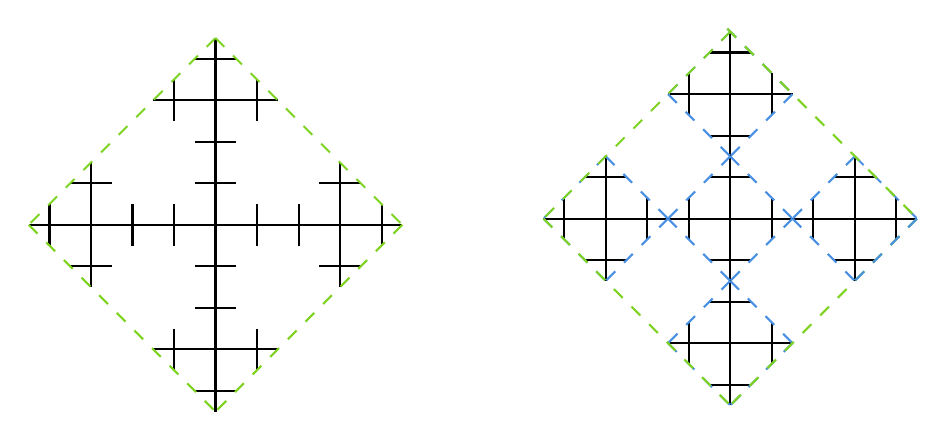
\begin{tikzpicture}[x=0.75pt,y=0.75pt,yscale=-1,xscale=1]
	%uncomment if require: \path (0,300); %set diagram left start at 0, and has height of 300
	
	%Straight Lines [id:da9355532760762474] 
	\draw    (144,170.67) -- (234,170.67) ;
	%Straight Lines [id:da5964144690386572] 
	\draw    (234,260.67) -- (234,170.67) ;
	%Straight Lines [id:da5166966545229968] 
	\draw    (234,170.67) -- (234,80.67) ;
	%Straight Lines [id:da7391858819502877] 
	\draw    (234,170.67) -- (324,170.67) ;
	%Straight Lines [id:da41589773867971025] 
	\draw    (294,140.67) -- (294,200.67) ;
	%Straight Lines [id:da4050702977235453] 
	\draw    (174,140.67) -- (174,200.67) ;
	%Straight Lines [id:da20582092340457592] 
	\draw    (204,230.67) -- (264,230.67) ;
	%Straight Lines [id:da7390405916041646] 
	\draw    (204,110.67) -- (264,110.67) ;
	%Straight Lines [id:da9899906610101565] 
	\draw    (164,150.67) -- (184,150.67) ;
	%Straight Lines [id:da41457128538077226] 
	\draw    (164,190.67) -- (184,190.67) ;
	%Straight Lines [id:da9932510119621577] 
	\draw    (224,210.67) -- (244,210.67) ;
	%Straight Lines [id:da570039755936011] 
	\draw    (224,190.67) -- (244,190.67) ;
	%Straight Lines [id:da9084396530899645] 
	\draw    (224,250.67) -- (244,250.67) ;
	%Straight Lines [id:da15309407933463914] 
	\draw    (284,190.67) -- (304,190.67) ;
	%Straight Lines [id:da13095833774901533] 
	\draw    (284,150.67) -- (304,150.67) ;
	%Straight Lines [id:da020887221653102972] 
	\draw    (224,150.67) -- (244,150.67) ;
	%Straight Lines [id:da7345561966712231] 
	\draw    (224,130.67) -- (244,130.67) ;
	%Straight Lines [id:da5362120333436483] 
	\draw    (224,90.67) -- (244,90.67) ;
	%Straight Lines [id:da7975638462661379] 
	\draw    (154,160.67) -- (154,180.67) ;
	%Straight Lines [id:da8143493857329925] 
	\draw    (194,160.67) -- (194,180.67) ;
	%Straight Lines [id:da6627411558310876] 
	\draw    (214,160.67) -- (214,180.67) ;
	%Straight Lines [id:da12362191876414352] 
	\draw    (254,160.67) -- (254,180.67) ;
	%Straight Lines [id:da7069540589636689] 
	\draw    (274,160.67) -- (274,180.67) ;
	%Straight Lines [id:da3928153922840286] 
	\draw    (314,160.67) -- (314,180.67) ;
	%Straight Lines [id:da2169381780841021] 
	\draw    (214,100.67) -- (214,120.67) ;
	%Straight Lines [id:da18731609764130341] 
	\draw    (254,100.67) -- (254,120.67) ;
	%Straight Lines [id:da38901588544180077] 
	\draw    (214,220.67) -- (214,240.67) ;
	%Straight Lines [id:da6421174062198961] 
	\draw    (254,220.67) -- (254,240.67) ;
	%Straight Lines [id:da12226658820871228] 
	%\draw [color={rgb, 255:red, 74; green, 144; blue, 226 }  ,draw opacity=1 ] [dash pattern={on 4.5pt off 4.5pt}]  (221,20) -- (191,50) ;
	%Straight Lines [id:da026721583537768434] 
	\draw [color={rgb, 255:red, 126; green, 211; blue, 33 }  ,draw opacity=1 ] [dash pattern={on 4.5pt off 4.5pt}]  (234,80.67) -- (324,170.67) ;
	%Straight Lines [id:da44767478808636885] 
	\draw [color={rgb, 255:red, 126; green, 211; blue, 33 }  ,draw opacity=1 ] [dash pattern={on 4.5pt off 4.5pt}]  (234,80.67) -- (144,170.67) ;
	%Straight Lines [id:da8112435482228784] 
	%\draw [color={rgb, 255:red, 74; green, 144; blue, 226 }  ,draw opacity=1 ] [dash pattern={on 4.5pt off 4.5pt}]  (321.4,78.2) -- (351.4,108.2) ;
	%Straight Lines [id:da23293877478548286] 
	\draw    (392,167.67) -- (482,167.67) ;
	%Straight Lines [id:da31990691332235865] 
	\draw    (482,257.67) -- (482,167.67) ;
	%Straight Lines [id:da13550842011059172] 
	\draw    (482,167.67) -- (482,77.67) ;
	%Straight Lines [id:da3786525368516451] 
	\draw    (482,167.67) -- (572,167.67) ;
	%Straight Lines [id:da23559495977997336] 
	\draw    (542,137.67) -- (542,197.67) ;
	%Straight Lines [id:da5695314439620682] 
	\draw    (422,137.67) -- (422,197.67) ;
	%Straight Lines [id:da19055834634380375] 
	\draw    (452,227.67) -- (512,227.67) ;
	%Straight Lines [id:da47149166103464524] 
	\draw    (452,107.67) -- (512,107.67) ;
	%Straight Lines [id:da025803623276352994] 
	\draw    (412,147.67) -- (432,147.67) ;
	%Straight Lines [id:da9002536538330218] 
	\draw    (412,187.67) -- (432,187.67) ;
	%Straight Lines [id:da3616034380123587] 
	\draw    (472,207.67) -- (492,207.67) ;
	%Straight Lines [id:da4659684911643208] 
	\draw    (472,187.67) -- (492,187.67) ;
	%Straight Lines [id:da6887240700183824] 
	\draw    (472,247.67) -- (492,247.67) ;
	%Straight Lines [id:da2075043300929269] 
	\draw    (532,187.67) -- (552,187.67) ;
	%Straight Lines [id:da7689395446852341] 
	\draw    (532,147.67) -- (552,147.67) ;
	%Straight Lines [id:da04283164908020154] 
	\draw    (472,147.67) -- (492,147.67) ;
	%Straight Lines [id:da7025075395144438] 
	\draw    (472,127.67) -- (492,127.67) ;
	%Straight Lines [id:da7129905877661015] 
	\draw    (472,87.67) -- (492,87.67) ;
	%Straight Lines [id:da13929958260781106] 
	\draw    (402,157.67) -- (402,177.67) ;
	%Straight Lines [id:da8805394368238584] 
	\draw    (442,157.67) -- (442,177.67) ;
	%Straight Lines [id:da9105517645243818] 
	\draw    (462,157.67) -- (462,177.67) ;
	%Straight Lines [id:da7375666971763377] 
	\draw    (502,157.67) -- (502,177.67) ;
	%Straight Lines [id:da519970374400013] 
	\draw    (522,157.67) -- (522,177.67) ;
	%Straight Lines [id:da9345793756328389] 
	\draw    (562,157.67) -- (562,177.67) ;
	%Straight Lines [id:da04789107971266471] 
	\draw    (462,97.67) -- (462,117.67) ;
	%Straight Lines [id:da1529122556111825] 
	\draw    (502,97.67) -- (502,117.67) ;
	%Straight Lines [id:da6146433793251727] 
	\draw    (462,217.67) -- (462,237.67) ;
	%Straight Lines [id:da494420762135248] 
	\draw    (502,217.67) -- (502,237.67) ;
	%Straight Lines [id:da495638130506715] 
	\draw [color={rgb, 255:red, 126; green, 211; blue, 33 }  ,draw opacity=1 ] [dash pattern={on 4.5pt off 4.5pt}]  (324,170.67) -- (234,260.67) ;
	%Straight Lines [id:da9417630463945195] 
	\draw [color={rgb, 255:red, 126; green, 211; blue, 33 }  ,draw opacity=1 ] [dash pattern={on 4.5pt off 4.5pt}]  (144,170.67) -- (234,260.67) ;
	%Straight Lines [id:da19448076333166897] 
	\draw [color={rgb, 255:red, 74; green, 144; blue, 226 }  ,draw opacity=1 ] [dash pattern={on 4.5pt off 4.5pt}]  (480.6,76.2) -- (510.6,106.2) ;
	%Straight Lines [id:da6966329371071581] 
	\draw [color={rgb, 255:red, 74; green, 144; blue, 226 }  ,draw opacity=1 ] [dash pattern={on 4.5pt off 4.5pt}]  (542,137.67) -- (572,167.67) ;
	%Straight Lines [id:da12519608396312176] 
	\draw [color={rgb, 255:red, 74; green, 144; blue, 226 }  ,draw opacity=1 ] [dash pattern={on 4.5pt off 4.5pt}]  (452,107.67) -- (482,137.67) ;
	%Straight Lines [id:da3844455078172324] 
	\draw [color={rgb, 255:red, 74; green, 144; blue, 226 }  ,draw opacity=1 ] [dash pattern={on 4.5pt off 4.5pt}]  (392,167.67) -- (422,197.67) ;
	%Straight Lines [id:da1083008562556157] 
	\draw [color={rgb, 255:red, 74; green, 144; blue, 226 }  ,draw opacity=1 ] [dash pattern={on 4.5pt off 4.5pt}]  (422,137.67) -- (452,167.67) ;
	%Straight Lines [id:da39018704416668093] 
	\draw [color={rgb, 255:red, 74; green, 144; blue, 226 }  ,draw opacity=1 ] [dash pattern={on 4.5pt off 4.5pt}]  (482,197.67) -- (512,227.67) ;
	%Straight Lines [id:da3591047819220503] 
	\draw [color={rgb, 255:red, 74; green, 144; blue, 226 }  ,draw opacity=1 ] [dash pattern={on 4.5pt off 4.5pt}]  (452,227.67) -- (482,257.67) ;
	%Straight Lines [id:da15564315798481743] 
	\draw [color={rgb, 255:red, 74; green, 144; blue, 226 }  ,draw opacity=1 ] [dash pattern={on 4.5pt off 4.5pt}]  (482,137.67) -- (512,167.67) ;
	%Straight Lines [id:da4754136960692654] 
	\draw [color={rgb, 255:red, 74; green, 144; blue, 226 }  ,draw opacity=1 ] [dash pattern={on 4.5pt off 4.5pt}]  (512,167.67) -- (542,197.67) ;
	%Straight Lines [id:da6921279716462709] 
	\draw [color={rgb, 255:red, 74; green, 144; blue, 226 }  ,draw opacity=1 ] [dash pattern={on 4.5pt off 4.5pt}]  (452,167.67) -- (482,197.67) ;
	%Straight Lines [id:da981122508969177] 
	\draw [color={rgb, 255:red, 74; green, 144; blue, 226 }  ,draw opacity=1 ] [dash pattern={on 4.5pt off 4.5pt}]  (422,137.67) -- (392,167.67) ;
	%Straight Lines [id:da3358448702724307] 
	\draw [color={rgb, 255:red, 74; green, 144; blue, 226 }  ,draw opacity=1 ] [dash pattern={on 4.5pt off 4.5pt}]  (452,167.67) -- (422,197.67) ;
	%Straight Lines [id:da3442244600026939] 
	\draw [color={rgb, 255:red, 74; green, 144; blue, 226 }  ,draw opacity=1 ] [dash pattern={on 4.5pt off 4.5pt}]  (512,107.67) -- (482,137.67) ;
	%Straight Lines [id:da6736183170796659] 
	\draw [color={rgb, 255:red, 74; green, 144; blue, 226 }  ,draw opacity=1 ] [dash pattern={on 4.5pt off 4.5pt}]  (482,77.67) -- (452,107.67) ;
	%Straight Lines [id:da38092812763972483] 
	\draw [color={rgb, 255:red, 74; green, 144; blue, 226 }  ,draw opacity=1 ] [dash pattern={on 4.5pt off 4.5pt}]  (542,137.67) -- (512,167.67) ;
	%Straight Lines [id:da43846868808333506] 
	\draw [color={rgb, 255:red, 74; green, 144; blue, 226 }  ,draw opacity=1 ] [dash pattern={on 4.5pt off 4.5pt}]  (482,197.67) -- (452,227.67) ;
	%Straight Lines [id:da438615072840856] 
	\draw [color={rgb, 255:red, 74; green, 144; blue, 226 }  ,draw opacity=1 ] [dash pattern={on 4.5pt off 4.5pt}]  (512,227.67) -- (482,257.67) ;
	%Straight Lines [id:da6064811902257697] 
	\draw [color={rgb, 255:red, 126; green, 211; blue, 33 }  ,draw opacity=1 ] [dash pattern={on 4.5pt off 4.5pt}]  (480.6,76.2) -- (570.6,166.2) ;
	%Straight Lines [id:da43605936381046007] 
	\draw [color={rgb, 255:red, 126; green, 211; blue, 33 }  ,draw opacity=1 ] [dash pattern={on 4.5pt off 4.5pt}]  (392,167.67) -- (482,257.67) ;
	%Straight Lines [id:da3042979851972285] 
	\draw [color={rgb, 255:red, 126; green, 211; blue, 33 }  ,draw opacity=1 ] [dash pattern={on 4.5pt off 4.5pt}]  (572,167.67) -- (482,257.67) ;
	%Straight Lines [id:da7604788032026776] 
	\draw [color={rgb, 255:red, 74; green, 144; blue, 226 }  ,draw opacity=1 ] [dash pattern={on 4.5pt off 4.5pt}]  (572,167.67) -- (542,197.67) ;
	%Straight Lines [id:da5827531272516981] 
	\draw [color={rgb, 255:red, 126; green, 211; blue, 33 }  ,draw opacity=1 ] [dash pattern={on 4.5pt off 4.5pt}]  (482,77.67) -- (392,167.67) ;
	%Straight Lines [id:da09759145386501367] 
	\draw [color={rgb, 255:red, 74; green, 144; blue, 226 }  ,draw opacity=1 ] [dash pattern={on 4.5pt off 4.5pt}]  (482,137.67) -- (452,167.67) ;
	%Straight Lines [id:da730504504375001] 
	\draw [color={rgb, 255:red, 74; green, 144; blue, 226 }  ,draw opacity=1 ] [dash pattern={on 4.5pt off 4.5pt}]  (512,167.67) -- (482,197.67) ;
	%Shape: Rectangle [id:dp3057385361936208] 
	%\draw  [draw opacity=0][fill={rgb, 255:red, 126; green, 211; blue, 33 }  ,fill opacity=0.21 ] (234,80.67) -- (324,170.67) -- (234,260.67) -- (144,170.67) -- cycle ;
	%Shape: Rectangle [id:dp9853880598725157] 
	%\draw  [draw opacity=0][fill={rgb, 255:red, 126; green, 211; blue, 33 }  ,fill opacity=0.21 ] (482,77.67) -- (572,167.67) -- (482,257.67) -- (392,167.67) -- cycle ;
	%Shape: Rectangle [id:dp036729546666227186] 
	%\draw  [draw opacity=0][fill={rgb, 255:red, 74; green, 144; blue, 226 }  ,fill opacity=0.37 ] (360,98.92) -- (390,128.92) -- (360,158.92) -- (330,128.92) -- cycle ;
	%Shape: Rectangle [id:dp06678489772991758] 
	%\draw  [draw opacity=0][fill={rgb, 255:red, 74; green, 144; blue, 226 }  ,fill opacity=0.37 ] (415.25,74.42) -- (445.25,104.42) -- (415.25,134.42) -- (385.25,104.42) -- cycle ;
	%Shape: Rectangle [id:dp3996131973661289] 
	%\draw  [draw opacity=0][fill={rgb, 255:red, 74; green, 144; blue, 226 }  ,fill opacity=0.37 ] (532.25,47.67) -- (562.25,77.67) -- (532.25,107.67) -- (502.25,77.67) -- cycle ;
	%Shape: Rectangle [id:dp41852476179520226] 
	%\draw  [draw opacity=0][fill={rgb, 255:red, 74; green, 144; blue, 226 }  ,fill opacity=0.37 ] (567.25,87.42) -- (597.25,117.42) -- (567.25,147.42) -- (537.25,117.42) -- cycle ;
	%Shape: Rectangle [id:dp19499344407905783] 
	%\draw  [draw opacity=0][fill={rgb, 255:red, 74; green, 144; blue, 226 }  ,fill opacity=0.37 ] (380,207.17) -- (410,237.17) -- (380,267.17) -- (350,237.17) -- cycle ;
\end{tikzpicture}
\caption{The opens sets $V$(green) and $\fracConst_i(V)$(blue)}
\end{figure}

Thus we can conclude from \cref{HausdorffDimTheorem} that 
\begin{equation}
	\sum_{i=1}^{5} \left(\frac{1}{3}\right)^{d_h} = 1 \Rightarrow \left(\frac{1}{3}\right)^{d_h} = \frac{1}{5} \Rightarrow d_h = \frac{\log 5}{\log 3}.
\end{equation}

Thus the Hausdorff dimension for the Vicsket set is $\log5/\log3$.

As stated earlier we will not be calculating the walk dimension, but instead just state it. The walk dimension for the Vicsek set is $d_w = d_h +1$. Thus we can make the following definition
\begin{defi}\label{defiDimensionsOfVicsek}
		The following constants hold for the Vicsek set $K$
		\begin{equation}
			d_h= \frac{\log 5}{\log 3}, \quad d_w = d_h +1, \quad \text{and} \quad d_s = \frac{d_h}{2d_w} = \frac{\log 5}{2 \log 15}
		\end{equation}
\end{defi}

Having just defined the Hausdorff dimension we will immediately use it to construct the following measure.
\begin{defi}\label{normalziedHausdorffMeasure}
	The normalized Hausdorff measure on $K$ which is given by the borel measure $\mu$ on $K$ such for any $i_1, \ldots i_n \in \cbr{1, \ldots, 5}$
	\begin{equation}
		\mu\left(\fracConst_{i_1} \circ \ldots \circ \fracConst_{i_n}(K)\right) = 5^{-n}.
	\end{equation}
\end{defi}

We have the following property of the measure $\mu$

\begin{prop}
	This measure $\mu$ is $d_h$-Ahlfors regular, i.e there exists $c_1, c_2 > 0$ such there for every $x \in K$ and $r \in [0, \diam(K)]$
	\begin{equation}
		c_1r^{d_h} \leq \mu(B(x,r)) \leq c_2 r^{d_h}.
	\end{equation}
\end{prop}
\begin{proof}
	If $r = 0$ the proof is obvious. So let $r \in (0, 1)$, and choose $n$ so $R \cd 3^{-(n+1)} \leq r \leq R \cd 3^{n}$ where $R = \diam(K)$. Note that for a sequence we have 
	$$\diam(\fracConst_{i_1} \circ \ldots \circ \fracConst_{i_{m}}(K))= 2\cd 3^{-m}\cd R.$$ 
	We can therefore construct a sequence $i_1, \ldots, i_n$ and $i_1, \ldots, i_{n+1}$ such that $B(x,r)\supset \fracConst_{i_1} \circ \ldots \circ \fracConst_{i_{n+1}}$ and $\fracConst_{i_1} \circ \ldots \circ \fracConst_{i_{n}} \cap B(x,r) \neq \emptyset$. Since $B(x,r)$ intersects with at most $5$ of these sequences we find an upper bound to be. 
	\begin{equation}
		\mu(B(x,r)) \leq 5\cd \mu\left(\fracConst_{i_1} \circ \ldots \circ \fracConst_{i_n}(K)\right) = 5\cd 5^{-n} = 5^2\cd5 ^{-(n+1)} \leq 5 \cd \left(R\cd 3^{-(n+1)}\right)^{d_h} \leq 5 \cd r^{d_h}.
	\end{equation} 
	thus we have an upper bound. This bound also works for $R < 1$ since then we just omit the constant from the calculations and have $3^{-(n+1)} \leq R^{-1}r$ and the bound becomes $5\cd \left(R^{-1} r\right)^{d_h}$. Likewise for the lower bound we have that there exists a sequence $i_1, \ldots i_{n+1}$ such that $B(x,r)\supset S_{i_1} \circ \ldots \circ S_{i_n}$ in which case
	\begin{equation}
		\mu(B(x,r)) \geq \left(\fracConst_{i_1} \circ \ldots \circ \fracConst_{i_{n+1}}(K)\right) = 5^{-(n+1)} \geq R\cd 5^{-(n+1)} \geq  5\cd \left(R^{-1}r\right)^{d_h}.
	\end{equation}
	Again this bound also holds for $R >1$ since we again omit $R$ in the calculations have $R^{-1}r \leq 3^{n}$ and the bound $5 \cd \left(R^{-r}r\right)^{d_h}$.
	
	Now assume $\diam(K) \geq r \geq 1$ the upper bound is simply $\mu(B(x,r)) \leq \mu(K) = 1 \leq r$. For the lower bound consider that there exists $m \in \nat$ so $3^{m-1}\leq  r \leq 3^{m}$, then
	\begin{equation}
		\mu(B(x,r)) \geq \mu(\fracConst_{i_1} \circ \ldots \circ \fracConst_{i_{m-1}}) = 5^{-(m-1)} = 5 \cd (3^{-m})^{d_h} \geq  (r3^{-2m})^{d_h}
	\end{equation}
	as desired.
\end{proof}

Next we have that we define a sequence of discrete measures 
\begin{defi}
	\begin{equation}\label{discreteMeasures}
		\mu_m = \frac{1}{a_m} \sum_{p \in V_m} \delta_p
	\end{equation}
	where $a_m = 5^{m}\cd 4 + 1$. 
\end{defi}

We have that $\mu_m \to \mu$ as $m \to \infty$, this follows from the fact that $\fracConst_i(K)$ "shrinks" the fractal down to $1/5$ the size around the point $p_i$. In which case for any sequence $i_1, \ldots i_n$ we have that
\begin{multline}
	\lim_{m \to \infty} \mu_m(\fracConst_{i_1},\circ \ldots \circ \fracConst_{i_n}(K)) = \lim_{m \to \infty}\frac{1}{a_m} \sum_{p \in V_m} \delta_p(\fracConst_{i_1},\circ \ldots \circ \fracConst_{i_n}(K)) \\ 
	= \lim_{m \to \infty} \frac{1}{a_m} \cd 5^{-n} \cd (5^{m}\cd 4 +1) = 5^{-n} = \mu(\fracConst_{i_1},\circ \ldots \circ \fracConst_{i_n}(K))
\end{multline}
Which leads us to the following corollary. \textcolor{red}{Wrote something wrong here maybe? wrt. to converge weakly vs converge in weak topology}
\begin{coro}\label{convergenceOfMeasures}
	The sequence of measure $(\mu_m)_{m \geq 0}$ defined in \eqref{discreteMeasures} converges weakly to the normalized Hausdorff measure $\mu$ on the Vicsek set $K$. That is
	\begin{equation}
		\lim_{m \to \infty} \int_{K}f \dd \mu_m = \int_{K} f \dd \mu
	\end{equation}
\end{coro}
 